\documentclass[varwidth=true, border=2pt]{standalone}
\usepackage{tkz-euclide}
\usepackage{tikz}
\usetikzlibrary{patterns}

\begin{document}
\usetkzobj{all}
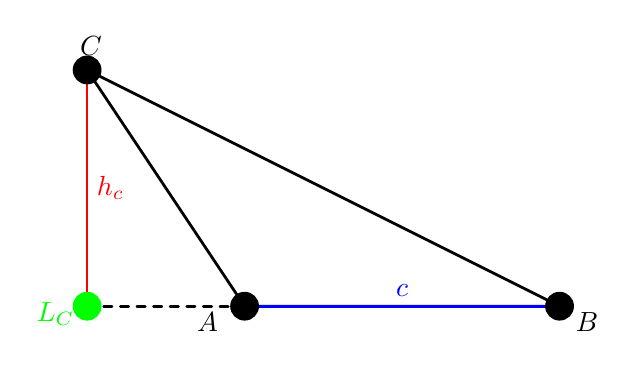
\begin{tikzpicture}
    \tkzSetUpPoint[shape=circle,size=10,color=black,fill=black]
    \tkzSetUpLine[line width=1]
    \tkzDefPoints{0/0/A, 4/0/B, -2/3/C}

    \tkzDefLine[orthogonal=through C,/tikz/overlay](A,B) \tkzGetPoint{helper}
    \tkzInterLL(A,B)(C,helper) \tkzGetPoint{Lc}

    %\tkzMarkAngle[arc=l,size=0.4cm,color=red,fill=red!20](A,La,B)
    %\tkzLabelAngle[pos=0.25](A,La,B){$\cdot$}

    \tkzDrawPolygon(A,B,C)

    \node at ($(A)+(-0.47,-0.2)$){$A$};
    \node at ($(B)+(0.35,-0.2)$) {$B$}; % \tkzLabelPoint[below](B){$B$} is not accurate enough
    \node at ($(C)+(0.05,0.3)$)  {$C$};
    \node[green] at ($(Lc)+(-0.4,-0.1)$)  {$L_C$};

    \tkzDrawSegments[red](C,Lc)
    \tkzDrawSegments[blue](A,B)
    \tkzDrawSegments[dashed](Lc,A)
    \tkzLabelSegment[right,red](C,Lc){$h_c$}
    \tkzLabelSegment[above,blue](A,B){$c$}
    \tkzDrawPoints(A,B,C)
    \tkzDrawPoints[color=green,fill=green](Lc)
\end{tikzpicture}
\end{document}
